\cajota{Tasa de denuncia de Violencia contra la mujer por departamento de registro}{\justifying A nivel nacional para el 2022 se reportó que 5 de cada 1,000 mujeres presentaron denuncias por delitos contemplados en la Ley Contra el Femicidio y Otras Formas de Violencia Contra de la Mujer.}{Tasa de denuncia de Violencia contra la mujer por departamento de registro,( 2022\footnote{Cifras preliminares.})}{República de Guatemala, Instituto Nacional de Estadística}{\begin{tikzpicture}[x=1pt,y=1pt, scale=1.75]% Created by tikzDevice version 0.12.4 on 2023-05-25 14:13:51
% !TEX encoding = UTF-8 Unicode
\definecolor{fillColor}{RGB}{255,255,255}
\path[use as bounding box,fill=fillColor,fill opacity=0.00] (0,0) rectangle (289.08,198.74);
\begin{scope}
\path[clip] (  0.00,  0.00) rectangle (289.08,198.74);

\path[] (  0.00,  0.00) rectangle (289.08,198.74);
\end{scope}
\begin{scope}
\path[clip] (  0.00,  0.00) rectangle (289.08,198.74);
\definecolor{drawColor}{RGB}{54,50,131}
\definecolor{fillColor}{RGB}{54,50,131}

\path[draw=drawColor,line width= 0.6pt,fill=fillColor] ( 59.47,  2.57) rectangle ( 60.32,  7.71);

\path[draw=drawColor,line width= 0.6pt,fill=fillColor] ( 59.47, 11.14) rectangle ( 64.23, 16.28);

\path[draw=drawColor,line width= 0.6pt,fill=fillColor] ( 59.47, 19.70) rectangle ( 69.03, 24.84);

\path[draw=drawColor,line width= 0.6pt,fill=fillColor] ( 59.47, 28.27) rectangle ( 69.26, 33.41);

\path[draw=drawColor,line width= 0.6pt,fill=fillColor] ( 59.47, 36.84) rectangle ( 71.74, 41.98);

\path[draw=drawColor,line width= 0.6pt,fill=fillColor] ( 59.47, 45.40) rectangle ( 74.80, 50.54);

\path[draw=drawColor,line width= 0.6pt,fill=fillColor] ( 59.47, 53.97) rectangle ( 79.50, 59.11);

\path[draw=drawColor,line width= 0.6pt,fill=fillColor] ( 59.47, 62.54) rectangle ( 80.72, 67.68);

\path[draw=drawColor,line width= 0.6pt,fill=fillColor] ( 59.47, 71.10) rectangle ( 82.94, 76.24);

\path[draw=drawColor,line width= 0.6pt,fill=fillColor] ( 59.47, 79.67) rectangle ( 83.52, 84.81);

\path[draw=drawColor,line width= 0.6pt,fill=fillColor] ( 59.47, 88.23) rectangle ( 86.35, 93.37);

\path[draw=color2,line width= 0.6pt,fill=color2] ( 59.47, 96.80) rectangle ( 86.47,101.94);

\path[draw=drawColor,line width= 0.6pt,fill=fillColor] ( 59.47,105.37) rectangle ( 88.02,110.51);

\path[draw=drawColor,line width= 0.6pt,fill=fillColor] ( 59.47,113.93) rectangle ( 95.69,119.07);

\path[draw=drawColor,line width= 0.6pt,fill=fillColor] ( 59.47,122.50) rectangle ( 98.04,127.64);

\path[draw=drawColor,line width= 0.6pt,fill=fillColor] ( 59.47,131.07) rectangle ( 99.33,136.21);

\path[draw=drawColor,line width= 0.6pt,fill=fillColor] ( 59.47,139.63) rectangle (100.04,144.77);

\path[draw=drawColor,line width= 0.6pt,fill=fillColor] ( 59.47,148.20) rectangle (103.70,153.34);

\path[draw=drawColor,line width= 0.6pt,fill=fillColor] ( 59.47,156.77) rectangle (108.72,161.91);

\path[draw=drawColor,line width= 0.6pt,fill=fillColor] ( 59.47,165.33) rectangle (114.67,170.47);

\path[draw=drawColor,line width= 0.6pt,fill=fillColor] ( 59.47,173.90) rectangle (124.91,179.04);

\path[draw=drawColor,line width= 0.6pt,fill=fillColor] ( 59.47,182.47) rectangle (144.92,187.61);

\path[draw=drawColor,line width= 0.6pt,fill=fillColor] ( 59.47,191.03) rectangle (261.39,196.17);
\definecolor{drawColor}{RGB}{0,0,0}

\path[draw=drawColor,line width= 0.1pt,line join=round] ( 59.47,-198.74) -- ( 59.47,397.48);

\node[text=drawColor,anchor=base west,inner sep=0pt, outer sep=0pt, scale=  1.02] at ( 62.56,  1.17) { 0.2};

\node[text=drawColor,anchor=base west,inner sep=0pt, outer sep=0pt, scale=  1.02] at ( 66.46,  9.74) { 0.9};

\node[text=drawColor,anchor=base west,inner sep=0pt, outer sep=0pt, scale=  1.02] at ( 71.27, 18.30) { 1.8};

\node[text=drawColor,anchor=base west,inner sep=0pt, outer sep=0pt, scale=  1.02] at ( 71.50, 26.87) { 1.8};

\node[text=drawColor,anchor=base west,inner sep=0pt, outer sep=0pt, scale=  1.02] at ( 73.97, 35.43) { 2.3};

\node[text=drawColor,anchor=base west,inner sep=0pt, outer sep=0pt, scale=  1.02] at ( 77.04, 44.00) { 2.9};

\node[text=drawColor,anchor=base west,inner sep=0pt, outer sep=0pt, scale=  1.02] at ( 81.73, 52.57) { 3.8};

\node[text=drawColor,anchor=base west,inner sep=0pt, outer sep=0pt, scale=  1.02] at ( 82.96, 61.13) { 4.0};

\node[text=drawColor,anchor=base west,inner sep=0pt, outer sep=0pt, scale=  1.02] at ( 85.18, 69.70) { 4.4};

\node[text=drawColor,anchor=base west,inner sep=0pt, outer sep=0pt, scale=  1.02] at ( 85.76, 78.27) { 4.5};

\node[text=drawColor,anchor=base west,inner sep=0pt, outer sep=0pt, scale=  1.02] at ( 88.59, 86.83) { 5.1};

\node[text=drawColor,anchor=base west,inner sep=0pt, outer sep=0pt, scale=  1.02] at ( 88.71, 95.40) { 5.1};

\node[text=drawColor,anchor=base west,inner sep=0pt, outer sep=0pt, scale=  1.02] at ( 90.26,103.97) { 5.4};

\node[text=drawColor,anchor=base west,inner sep=0pt, outer sep=0pt, scale=  1.02] at ( 97.93,112.53) { 6.8};

\node[text=drawColor,anchor=base west,inner sep=0pt, outer sep=0pt, scale=  1.02] at (100.28,121.10) { 7.3};

\node[text=drawColor,anchor=base west,inner sep=0pt, outer sep=0pt, scale=  1.02] at (101.57,129.67) { 7.5};

\node[text=drawColor,anchor=base west,inner sep=0pt, outer sep=0pt, scale=  1.02] at (102.28,138.23) { 7.7};

\node[text=drawColor,anchor=base west,inner sep=0pt, outer sep=0pt, scale=  1.02] at (105.93,146.80) { 8.3};

\node[text=drawColor,anchor=base west,inner sep=0pt, outer sep=0pt, scale=  1.02] at (110.96,155.37) { 9.3};

\node[text=drawColor,anchor=base west,inner sep=0pt, outer sep=0pt, scale=  1.02] at (117.80,163.93) {10.4};

\node[text=drawColor,anchor=base west,inner sep=0pt, outer sep=0pt, scale=  1.02] at (128.04,172.50) {12.4};

\node[text=drawColor,anchor=base west,inner sep=0pt, outer sep=0pt, scale=  1.02] at (148.05,181.07) {16.1};

\node[text=drawColor,anchor=base west,inner sep=0pt, outer sep=0pt, scale=  1.02] at (264.52,189.63) {38.1};

\path[] ( 59.47,  0.00) rectangle (261.39,198.74);

\path[] ( 59.47,  5.14) --
	(261.39,  5.14);

\path[] ( 59.47, 13.71) --
	(261.39, 13.71);

\path[] ( 59.47, 22.27) --
	(261.39, 22.27);

\path[] ( 59.47, 30.84) --
	(261.39, 30.84);

\path[] ( 59.47, 39.41) --
	(261.39, 39.41);

\path[] ( 59.47, 47.97) --
	(261.39, 47.97);

\path[] ( 59.47, 56.54) --
	(261.39, 56.54);

\path[] ( 59.47, 65.11) --
	(261.39, 65.11);

\path[] ( 59.47, 73.67) --
	(261.39, 73.67);

\path[] ( 59.47, 82.24) --
	(261.39, 82.24);

\path[] ( 59.47, 90.80) --
	(261.39, 90.80);

\path[] ( 59.47, 99.37) --
	(261.39, 99.37);

\path[] ( 59.47,107.94) --
	(261.39,107.94);

\path[] ( 59.47,116.50) --
	(261.39,116.50);

\path[] ( 59.47,125.07) --
	(261.39,125.07);

\path[] ( 59.47,133.64) --
	(261.39,133.64);

\path[] ( 59.47,142.20) --
	(261.39,142.20);

\path[] ( 59.47,150.77) --
	(261.39,150.77);

\path[] ( 59.47,159.34) --
	(261.39,159.34);

\path[] ( 59.47,167.90) --
	(261.39,167.90);

\path[] ( 59.47,176.47) --
	(261.39,176.47);

\path[] ( 59.47,185.04) --
	(261.39,185.04);

\path[] ( 59.47,193.60) --
	(261.39,193.60);

\path[] ( 59.47,  0.00) rectangle (261.39,198.74);
\end{scope}
\begin{scope}
\path[clip] (  0.00,  0.00) rectangle (289.08,198.74);

\path[] ( 59.47,  0.00) --
	( 59.47,198.74);
\end{scope}
\begin{scope}
\path[clip] (  0.00,  0.00) rectangle (289.08,198.74);
\definecolor{drawColor}{RGB}{0,0,0}

\node[text=drawColor,anchor=base east,inner sep=0pt, outer sep=0pt, scale=  1.00] at ( 56.72,  1.23) {Alta Verapaz };

\node[text=drawColor,anchor=base east,inner sep=0pt, outer sep=0pt, scale=  1.00] at ( 56.72,  9.80) {Quiché };

\node[text=drawColor,anchor=base east,inner sep=0pt, outer sep=0pt, scale=  1.00] at ( 56.72, 18.36) {Jalapa };

\node[text=drawColor,anchor=base east,inner sep=0pt, outer sep=0pt, scale=  1.00] at ( 56.72, 26.93) {Huehuetenango };

\node[text=drawColor,anchor=base east,inner sep=0pt, outer sep=0pt, scale=  1.00] at ( 56.72, 35.50) {San Marcos };

\node[text=drawColor,anchor=base east,inner sep=0pt, outer sep=0pt, scale=  1.00] at ( 56.72, 44.06) {Quetzaltenango };

\node[text=drawColor,anchor=base east,inner sep=0pt, outer sep=0pt, scale=  1.00] at ( 56.72, 52.63) {Chiquimula };

\node[text=drawColor,anchor=base east,inner sep=0pt, outer sep=0pt, scale=  1.00] at ( 56.72, 61.20) {Suchitepéquez };

\node[text=drawColor,anchor=base east,inner sep=0pt, outer sep=0pt, scale=  1.00] at ( 56.72, 69.76) {Sololá };

\node[text=drawColor,anchor=base east,inner sep=0pt, outer sep=0pt, scale=  1.00] at ( 56.72, 78.33) {Petén };

\node[text=drawColor,anchor=base east,inner sep=0pt, outer sep=0pt, scale=  1.00] at ( 56.72, 86.90) {Guatemala };

\node[text=drawColor,anchor=base east,inner sep=0pt, outer sep=0pt, scale=  1.00] at ( 56.72, 95.46) {Nacional};

\node[text=drawColor,anchor=base east,inner sep=0pt, outer sep=0pt, scale=  1.00] at ( 56.72,104.03) {Escuintla };

\node[text=drawColor,anchor=base east,inner sep=0pt, outer sep=0pt, scale=  1.00] at ( 56.72,112.60) {Santa Rosa };

\node[text=drawColor,anchor=base east,inner sep=0pt, outer sep=0pt, scale=  1.00] at ( 56.72,121.16) {Retalhuleu };

\node[text=drawColor,anchor=base east,inner sep=0pt, outer sep=0pt, scale=  1.00] at ( 56.72,129.73) {Zacapa };

\node[text=drawColor,anchor=base east,inner sep=0pt, outer sep=0pt, scale=  1.00] at ( 56.72,138.30) {Jutiapa };

\node[text=drawColor,anchor=base east,inner sep=0pt, outer sep=0pt, scale=  1.00] at ( 56.72,146.86) {Chimaltenango };

\node[text=drawColor,anchor=base east,inner sep=0pt, outer sep=0pt, scale=  1.00] at ( 56.72,155.43) {Sacatepéquez };

\node[text=drawColor,anchor=base east,inner sep=0pt, outer sep=0pt, scale=  1.00] at ( 56.72,163.99) {Baja Verapaz };

\node[text=drawColor,anchor=base east,inner sep=0pt, outer sep=0pt, scale=  1.00] at ( 56.72,172.56) {Totonicapán };

\node[text=drawColor,anchor=base east,inner sep=0pt, outer sep=0pt, scale=  1.00] at ( 56.72,181.13) {Izabal };

\node[text=drawColor,anchor=base east,inner sep=0pt, outer sep=0pt, scale=  1.00] at ( 56.72,189.69) {El Progreso };
\end{scope}
\begin{scope}
\path[clip] (  0.00,  0.00) rectangle (289.08,198.74);

\path[] ( 56.72,  5.14) --
	( 59.47,  5.14);

\path[] ( 56.72, 13.71) --
	( 59.47, 13.71);

\path[] ( 56.72, 22.27) --
	( 59.47, 22.27);

\path[] ( 56.72, 30.84) --
	( 59.47, 30.84);

\path[] ( 56.72, 39.41) --
	( 59.47, 39.41);

\path[] ( 56.72, 47.97) --
	( 59.47, 47.97);

\path[] ( 56.72, 56.54) --
	( 59.47, 56.54);

\path[] ( 56.72, 65.11) --
	( 59.47, 65.11);

\path[] ( 56.72, 73.67) --
	( 59.47, 73.67);

\path[] ( 56.72, 82.24) --
	( 59.47, 82.24);

\path[] ( 56.72, 90.80) --
	( 59.47, 90.80);

\path[] ( 56.72, 99.37) --
	( 59.47, 99.37);

\path[] ( 56.72,107.94) --
	( 59.47,107.94);

\path[] ( 56.72,116.50) --
	( 59.47,116.50);

\path[] ( 56.72,125.07) --
	( 59.47,125.07);

\path[] ( 56.72,133.64) --
	( 59.47,133.64);

\path[] ( 56.72,142.20) --
	( 59.47,142.20);

\path[] ( 56.72,150.77) --
	( 59.47,150.77);

\path[] ( 56.72,159.34) --
	( 59.47,159.34);

\path[] ( 56.72,167.90) --
	( 59.47,167.90);

\path[] ( 56.72,176.47) --
	( 59.47,176.47);

\path[] ( 56.72,185.04) --
	( 59.47,185.04);

\path[] ( 56.72,193.60) --
	( 59.47,193.60);
\end{scope}
\begin{scope}
\path[clip] (  0.00,  0.00) rectangle (289.08,198.74);

\path[] ( 59.47,  0.00) --
	(261.39,  0.00);
\end{scope}
\end{tikzpicture}}{INE - Datos proporcionados por el Ministerio Público 2022}

\cajota{Denuncias por los delitos contemplados en la Ley Contra el Femicidio y Otras Formas de Violencia Contra a la Mujer por departamento de registro}{\\[-1.7cm]\input{Descripciones/des5_02.tex}}{Denuncias por los delitos contemplados en la Ley Contra el Femicidio y Otras Formas de Violencia Contra a la Mujer por departamento de registro, (2022\footnote{Cifras preliminares.})}{República de Guatemala, Instituto Nacional de Estadística}{\\[-1.7cm]\resizebox{\textwidth}{!}{\begin{tabular}[t]{cccccccc}
\toprule
\textbf{Tipo de delito (violencia)} & \textbf{Guatemala} & \textbf{El Progreso} & \textbf{Sacatepéquez} & \textbf{Chimaltenango} & \textbf{Quiché} & \textbf{Santa Rosa} & \textbf{Quetzaltenango}\\
\midrule
\cellcolor[HTML]{B6B3FF}{Psicológica} & \cellcolor[HTML]{B6B3FF}{3,097} & \cellcolor[HTML]{B6B3FF}{1,362} & \cellcolor[HTML]{B6B3FF}{695} & \cellcolor[HTML]{B6B3FF}{1,231} & \cellcolor[HTML]{B6B3FF}{77} & \cellcolor[HTML]{B6B3FF}{633} & \cellcolor[HTML]{B6B3FF}{687}\\
Física & 2,271 & 1,225 & 252 & 1,073 & 243 & 480 & 242\\
\cellcolor[HTML]{B6B3FF}{Física y psicológica} & \cellcolor[HTML]{B6B3FF}{1,913} & \cellcolor[HTML]{B6B3FF}{546} & \cellcolor[HTML]{B6B3FF}{597} & \cellcolor[HTML]{B6B3FF}{560} & \cellcolor[HTML]{B6B3FF}{98} & \cellcolor[HTML]{B6B3FF}{276} & \cellcolor[HTML]{B6B3FF}{316}\\
VCM\footnote{VCM: incluye casos que no reportaron desagregación por tipo de violencia.}. & 2,022 & 477 & 233 & 169 & 70 & 92 & 83\\
\cellcolor[HTML]{B6B3FF}{Psicológica y económica} & \cellcolor[HTML]{B6B3FF}{58} & \cellcolor[HTML]{B6B3FF}{56} & \cellcolor[HTML]{B6B3FF}{70} & \cellcolor[HTML]{B6B3FF}{44} & \cellcolor[HTML]{B6B3FF}{3} & \cellcolor[HTML]{B6B3FF}{28} & \cellcolor[HTML]{B6B3FF}{24}\\
Física, psicológica y económica & 46 & 34 & 36 & 14 & 5 & 13 & 32\\
\cellcolor[HTML]{B6B3FF}{VCM y económica} & \cellcolor[HTML]{B6B3FF}{45} & \cellcolor[HTML]{B6B3FF}{41} & \cellcolor[HTML]{B6B3FF}{14} & \cellcolor[HTML]{B6B3FF}{48} & \cellcolor[HTML]{B6B3FF}{3} & \cellcolor[HTML]{B6B3FF}{31} & \cellcolor[HTML]{B6B3FF}{18}\\
Femicidio & 27 & 5 & 4 & 11 & 3 & 4 & 7\\
\cellcolor[HTML]{B6B3FF}{Física y económica} & \cellcolor[HTML]{B6B3FF}{9} & \cellcolor[HTML]{B6B3FF}{13} & \cellcolor[HTML]{B6B3FF}{0} & \cellcolor[HTML]{B6B3FF}{5} & \cellcolor[HTML]{B6B3FF}{3} & \cellcolor[HTML]{B6B3FF}{4} & \cellcolor[HTML]{B6B3FF}{2}\\
Otros tipos & 74 & 36 & 25 & 27 & 6 & 22 & 23\\
\bottomrule
\end{tabular}}
\\[0.5cm]
\resizebox{\textwidth}{!}{\begin{tabular}[t]{ccccccccc}
	\toprule
	\textbf{Tipo de delito (violencia)} &            & \textbf{Totonicapán} & \textbf{Sololá} & \textbf{Suchitepéquez} & \textbf{Petén} & \textbf{San Marcos} & \textbf{Huehuetenango} & \textbf{Escuintla}\\
	\midrule
	\cellcolor[HTML]{B6B3FF}{Psicológica} & \cellcolor[HTML]{B6B3FF}{ } & \cellcolor[HTML]{B6B3FF}{1,063} & \cellcolor[HTML]{B6B3FF}{471} & \cellcolor[HTML]{B6B3FF}{487} & \cellcolor[HTML]{B6B3FF}{630} & \cellcolor[HTML]{B6B3FF}{822} & \cellcolor[HTML]{B6B3FF}{724} & \cellcolor[HTML]{B6B3FF}{651}\\
	Física & & 862 & 260 & 84 & 309 & 50 & 233 & 710\\
	\cellcolor[HTML]{B6B3FF}{Física y psicológica} & \cellcolor[HTML]{B6B3FF}{} & \cellcolor[HTML]{B6B3FF}{768} & \cellcolor[HTML]{B6B3FF}{111} & \cellcolor[HTML]{B6B3FF}{494} & \cellcolor[HTML]{B6B3FF}{314} & \cellcolor[HTML]{B6B3FF}{257} & \cellcolor[HTML]{B6B3FF}{211} & \cellcolor[HTML]{B6B3FF}{444}\\
	VCM & & 366 & 161 & 128 & 73 & 255 & 106 & 295\\
	\cellcolor[HTML]{B6B3FF}{Psicológica y económica} & \cellcolor[HTML]{B6B3FF}{} & \cellcolor[HTML]{B6B3FF}{71} & \cellcolor[HTML]{B6B3FF}{14} & \cellcolor[HTML]{B6B3FF}{25} & \cellcolor[HTML]{B6B3FF}{19} & \cellcolor[HTML]{B6B3FF}{14} & \cellcolor[HTML]{B6B3FF}{27} & \cellcolor[HTML]{B6B3FF}{7}\\
	Física, psicológica y económica & & 50 & 17 & 23 & 20 & 19 & 13 & 8\\
	\cellcolor[HTML]{B6B3FF}{VCM y económica} & \cellcolor[HTML]{B6B3FF}{} & \cellcolor[HTML]{B6B3FF}{36} & \cellcolor[HTML]{B6B3FF}{4} & \cellcolor[HTML]{B6B3FF}{8} & \cellcolor[HTML]{B6B3FF}{12} & \cellcolor[HTML]{B6B3FF}{3} & \cellcolor[HTML]{B6B3FF}{6} & \cellcolor[HTML]{B6B3FF}{16}\\
	Femicidio & & 6 & 1 & 3 & 3 & 2 & 13 & 6\\
	\cellcolor[HTML]{B6B3FF}{Física y económica} & \cellcolor[HTML]{B6B3FF}{} & \cellcolor[HTML]{B6B3FF}{22} & \cellcolor[HTML]{B6B3FF}{3} & \cellcolor[HTML]{B6B3FF}{3} & \cellcolor[HTML]{B6B3FF}{6} & \cellcolor[HTML]{B6B3FF}{1} & \cellcolor[HTML]{B6B3FF}{0} & \cellcolor[HTML]{B6B3FF}{14}\\
	Otros tipos & & 35 & 53 & 13 & 25 & 16 & 27 & 18\\
	\bottomrule
\end{tabular}}
\\[0.5cm]
\resizebox{\textwidth}{!}{\begin{tabular}[t]{cccccccccc}
	\toprule
	\textbf{Tipo de delito (violencia)} &        & \textbf{Baja Verapaz} & \textbf{Alta Verapaz} & \textbf{Retalhuleu} & \textbf{Izabal} & \textbf{Zacapa} & \textbf{Chiquimula} & \textbf{Jalapa} & \textbf{Jutiapa} \\
	\midrule
	\cellcolor[HTML]{B6B3FF}{Psicológica} & \cellcolor[HTML]{B6B3FF}{ } & \cellcolor[HTML]{B6B3FF}{877} & \cellcolor[HTML]{B6B3FF}{579} & \cellcolor[HTML]{B6B3FF}{630} & \cellcolor[HTML]{B6B3FF}{1,631} & \cellcolor[HTML]{B6B3FF}{426} & \cellcolor[HTML]{B6B3FF}{408} & \cellcolor[HTML]{B6B3FF}{125} & \cellcolor[HTML]{B6B3FF}{757}\\
	Física &  & 177 & 71 & 257 & 412 & 238 & 211 & 117 & 555\\
	\cellcolor[HTML]{B6B3FF}{Física y psicológica} & \cellcolor[HTML]{B6B3FF}{ } & \cellcolor[HTML]{B6B3FF}{399} & \cellcolor[HTML]{B6B3FF}{0} & \cellcolor[HTML]{B6B3FF}{152} & \cellcolor[HTML]{B6B3FF}{1,014} & \cellcolor[HTML]{B6B3FF}{267} & \cellcolor[HTML]{B6B3FF}{158} & \cellcolor[HTML]{B6B3FF}{84} & \cellcolor[HTML]{B6B3FF}{599}\\
	VCM &  & 305 & 20 & 380 & 455 & 62 & 58 & 28 & 157\\
	\cellcolor[HTML]{B6B3FF}{Psicológica y económica} & \cellcolor[HTML]{B6B3FF}{ } & \cellcolor[HTML]{B6B3FF}{22} & \cellcolor[HTML]{B6B3FF}{1} & \cellcolor[HTML]{B6B3FF}{12} & \cellcolor[HTML]{B6B3FF}{49} & \cellcolor[HTML]{B6B3FF}{14} & \cellcolor[HTML]{B6B3FF}{10} & \cellcolor[HTML]{B6B3FF}{5} & \cellcolor[HTML]{B6B3FF}{32}\\
	Física, psicológica y económica &  & 10 & 2 & 11 & 56 & 13 & 15 & 6 & 13\\
	\cellcolor[HTML]{B6B3FF}{VCM y económica} & \cellcolor[HTML]{B6B3FF}{ } & \cellcolor[HTML]{B6B3FF}{3} & \cellcolor[HTML]{B6B3FF}{3} & \cellcolor[HTML]{B6B3FF}{8} & \cellcolor[HTML]{B6B3FF}{9} & \cellcolor[HTML]{B6B3FF}{3} & \cellcolor[HTML]{B6B3FF}{3} & \cellcolor[HTML]{B6B3FF}{4} & \cellcolor[HTML]{B6B3FF}{16}\\
	Femicidio &  & 11 & 0 & 5 & 8 & 8 & 1 & 4 & 12\\
	\cellcolor[HTML]{B6B3FF}{Física y económica} & \cellcolor[HTML]{B6B3FF}{ } & \cellcolor[HTML]{B6B3FF}{0} & \cellcolor[HTML]{B6B3FF}{0} & \cellcolor[HTML]{B6B3FF}{1} & \cellcolor[HTML]{B6B3FF}{10} & \cellcolor[HTML]{B6B3FF}{8} & \cellcolor[HTML]{B6B3FF}{5} & \cellcolor[HTML]{B6B3FF}{2} & \cellcolor[HTML]{B6B3FF}{9}\\
	Otros tipos &  & 10 & 2 & 10 & 56 & 21 & 27 & 3 & 20\\
	\bottomrule
\end{tabular}}
}{INE - Datos proporcionados por el Ministerio Público 2022}{}

\cajota{Denuncias por los delitos contemplados en la Ley Contra el Femicidio y Otras Formas de Violencia Contra a la Mujer, según grupos de edad}{La tabla muestra el número de denuncias realizadas en el Ministerio Público durante el 2022 por tipo de delito contemplados en la Ley Contra el Femicidio y Otras Formas de Violencia Contra la Mujer, según grupos de edad.

Para 2022, se reportaron 17,447 denuncias por violencia psicológica, de las cuales 5,921 fueron hacia mujeres de 30 a 44 años y 5,765 de mujeres de 15 a 29 años. Así mismo, se reportaron 10,332 denuncias por violencia física, de las cuales 4,080 se dieron a mujeres de 15 a 29 años y 3,398 a mujeres de 30 a 44 años. }{Denuncias por los delitos contemplados en la Ley Contra el Femicidio y Otras Formas de Violencia Contra a la Mujer, según grupos de edad, (2022\footnote{Cifras preliminares.})}{República de Guatemala, Instituto Nacional de Estadística}{\begin{tabular}[t]{ccccccc}
\toprule
\multicolumn{1}{c}{\textbf{ }} & \multicolumn{5}{c}{\textbf{Grupos de edad}} & \multicolumn{1}{c}{\textbf{ }} \\
\cmidrule(l{3pt}r{3pt}){2-6}
\textbf{Tipo de delito} & \textbf{0-14} & \textbf{15-29} & \textbf{30-44} & \textbf{45-64} & \textbf{65+} & \textbf{Ignorado}\\
\midrule
\cellcolor[HTML]{A8A4FB}{Psicológica} & \cellcolor[HTML]{A8A4FB}{58} & \cellcolor[HTML]{A8A4FB}{5,765} & \cellcolor[HTML]{A8A4FB}{5,921} & \cellcolor[HTML]{A8A4FB}{2,193} & \cellcolor[HTML]{A8A4FB}{348} & \cellcolor[HTML]{A8A4FB}{3,162}\\
Física & 45 & 4,080 & 3,398 & 932 & 119 & 1,758\\
\cellcolor[HTML]{A8A4FB}{Física y psicológica} & \cellcolor[HTML]{A8A4FB}{35} & \cellcolor[HTML]{A8A4FB}{3,841} & \cellcolor[HTML]{A8A4FB}{3,011} & \cellcolor[HTML]{A8A4FB}{829} & \cellcolor[HTML]{A8A4FB}{90} & \cellcolor[HTML]{A8A4FB}{1,772}\\
VCM\footnote{Violencia contra la mujer incluye casos que no reportaron desagregación por tipo de violencia.} & 16 & 1,958 & 2,009 & 868 & 149 & 995\\
\cellcolor[HTML]{A8A4FB}{Psicológica y económica} & \cellcolor[HTML]{A8A4FB}{0} & \cellcolor[HTML]{A8A4FB}{183} & \cellcolor[HTML]{A8A4FB}{221} & \cellcolor[HTML]{A8A4FB}{89} & \cellcolor[HTML]{A8A4FB}{23} & \cellcolor[HTML]{A8A4FB}{89}\\
Física, psicológica y económica & 3 & 181 & 143 & 35 & 5 & 89\\
\cellcolor[HTML]{A8A4FB}{VCM y económica} & \cellcolor[HTML]{A8A4FB}{0} & \cellcolor[HTML]{A8A4FB}{96} & \cellcolor[HTML]{A8A4FB}{124} & \cellcolor[HTML]{A8A4FB}{50} & \cellcolor[HTML]{A8A4FB}{6} & \cellcolor[HTML]{A8A4FB}{58}\\
Femicidio & 6 & 44 & 41 & 19 & 2 & 32\\
\cellcolor[HTML]{A8A4FB}{Física y económica} & \cellcolor[HTML]{A8A4FB}{1} & \cellcolor[HTML]{A8A4FB}{46} & \cellcolor[HTML]{A8A4FB}{42} & \cellcolor[HTML]{A8A4FB}{10} & \cellcolor[HTML]{A8A4FB}{0} & \cellcolor[HTML]{A8A4FB}{21}\\
Otros tipos & 17 & 209 & 190 & 53 & 7 & 73\\
\bottomrule
\end{tabular}
}{INE - Datos proporcionados por el Ministerio Público 2022}{}

\cajota{Denuncia por los delitos contemplados en la Ley Contra el Femicidio y Otras Formas de Violencia Contra a la Mujer, según Pueblo}{La tabla muestra las denuncicas que se reportaron por tipo de delito contempladas en la Ley Contra el Femicidio y Otras Formas de Violencia Contra la Mujer por pueblo de pertenencia en el Ministerio Público durante el 2022. 

Durante el 2022, se reportaron 45,560 denuncias por violencia en contra de mujeres, de las cuales solo en 341 de las denuncias se identificó el pueblo de pertenencia.
}{Denuncia por los delitos contemplados en la Ley Contra el Femicidio y Otras Formas de Violencia Contra a la Mujer, según Pueblos, (2022\footnote{Cifras preliminares.})}{República de Guatemala, Instituto Nacional de Estadística}{\begin{tabular}[t]{ccccc}
\toprule
\multicolumn{1}{c}{\textbf{ }} & \multicolumn{2}{c}{\textbf{2018}} & \multicolumn{2}{c}{\textbf{2022*}} \\
\cmidrule(l{3pt}r{3pt}){2-3} \cmidrule(l{3pt}r{3pt}){4-5}
\textbf{Pueblo} & \textbf{Mujeres} & \textbf{Hombres} & \textbf{Mujeres} & \textbf{Hombres}\\
\midrule
\cellcolor[HTML]{B6B3FF}{Ladinos(as)} & \cellcolor[HTML]{B6B3FF}{14320} & \cellcolor[HTML]{B6B3FF}{2118} & \cellcolor[HTML]{B6B3FF}{3315} & \cellcolor[HTML]{B6B3FF}{19133}\\
Maya & 7650 & 1137 & 1517 & 8609\\
\cellcolor[HTML]{B6B3FF}{Garifuna} & \cellcolor[HTML]{B6B3FF}{46} & \cellcolor[HTML]{B6B3FF}{11} & \cellcolor[HTML]{B6B3FF}{6} & \cellcolor[HTML]{B6B3FF}{40}\\
Xinca & 37 & 12 & 14 & 35\\
\cellcolor[HTML]{B6B3FF}{Otro} & \cellcolor[HTML]{B6B3FF}{91} & \cellcolor[HTML]{B6B3FF}{10} & \cellcolor[HTML]{B6B3FF}{25} & \cellcolor[HTML]{B6B3FF}{152}\\
No indica & 3876 & 421 & 477 & 3369\\
\cellcolor[HTML]{B6B3FF}{Ignorado} & \cellcolor[HTML]{B6B3FF}{234} & \cellcolor[HTML]{B6B3FF}{29} & \cellcolor[HTML]{B6B3FF}{102} & \cellcolor[HTML]{B6B3FF}{400}\\
\bottomrule
\end{tabular}
}{INE - Datos proporcionados por el Ministerio Público 2022}{}

\cajita{Mujeres víctimas de violencia contra la mujer, según Pueblos }{La tabla muestra el número de mujeres víctimas por hechos de violencia contemplados en los delitos de la Ley Contra el Femicidio y Otras Formas de Violencia Contra la Mujer durante 2018 y 2022. 

De 2018 a 2022 en los datos del Ministerio Público en la categoría de pueblo registró como ignorado a 181,532 mujeres víctimas de violencia contra la mujer, de los cuales 40,001 se registraron en 2022. }{Mujeres víctimas de violencia contra la mujer, según Pueblos (2018 - 2022\footnote{Información preliminar, la variación en las cifras de los registros de 2022, de acuerdo a lo indicado por el Ministerio Público se debe a la actualización de su Sistema Informático.})}{República de Guatemala, Instituto Nacional de Estadística}{\begin{tabular}[t]{cccccc}
\toprule
\textbf{Pueblo} & \textbf{2018} & \textbf{2019} & \textbf{2020} & \textbf{2021} & \textbf{2022}\\
\midrule
\cellcolor[HTML]{A8A4FB}{Ladino} & \cellcolor[HTML]{A8A4FB}{10,367} & \cellcolor[HTML]{A8A4FB}{11,480} & \cellcolor[HTML]{A8A4FB}{9,608} & \cellcolor[HTML]{A8A4FB}{12,291} & \cellcolor[HTML]{A8A4FB}{222}\\
Maya & 3,471 & 3,814 & 3,874 & 3,816 & 6\\
\cellcolor[HTML]{A8A4FB}{Garífuna} & \cellcolor[HTML]{A8A4FB}{11} & \cellcolor[HTML]{A8A4FB}{18} & \cellcolor[HTML]{A8A4FB}{32} & \cellcolor[HTML]{A8A4FB}{16} & \cellcolor[HTML]{A8A4FB}{1}\\
Xinka & 10 & 45 & 23 & 9 & NA\\
\cellcolor[HTML]{A8A4FB}{Otro} & \cellcolor[HTML]{A8A4FB}{947} & \cellcolor[HTML]{A8A4FB}{1,150} & \cellcolor[HTML]{A8A4FB}{1299} & \cellcolor[HTML]{A8A4FB}{1,008} & \cellcolor[HTML]{A8A4FB}{55}\\
No indica & 701 & 715 & 308 & 303 & 2\\
\cellcolor[HTML]{A8A4FB}{Ignorado} & \cellcolor[HTML]{A8A4FB}{31,963} & \cellcolor[HTML]{A8A4FB}{34,982} & \cellcolor[HTML]{A8A4FB}{37,295} & \cellcolor[HTML]{A8A4FB}{37,291} & \cellcolor[HTML]{A8A4FB}{40,001}\\
\bottomrule
\end{tabular}
}{INE - Datos proporcionados por el Ministerio Público 2022}{}

\cajita{Mujeres víctimas de violencia contra la mujer, según tipo de violencia sufrida }{La tabla muestra el número de mujeres víctimas violencia según los tipos de violencia contemplados en la ley contra el femicidio y otras formas de violencia contra la mujer del 2018 a 2022. 

Durante el 2018 y 2022 se registró 87,911 mujeres víctimas de violencia psicológica de las cuales 19,357 se reportaron en el 2019 y 15,297 en el 2022. 

Durante el 2018 y 2022 se registró 44,770 mujeres víctimas de violencia física de las cuales 11,406 se reportaron en el 2018 y 6,056 en el 2021. 
}{Mujeres víctimas de violencia contra la mujer, según tipo de violencia sufrida (2018 - 2022\footnote{Cifras preliminares.})}{República de Guatemala, Instituto Nacional de Estadística}{\begin{tabular}[t]{cccccc}
\toprule
\textbf{Tipo de violencia} & \textbf{2018} & \textbf{2019} & \textbf{2020} & \textbf{2021} & \textbf{2022}\\
\midrule
\cellcolor[HTML]{B6B3FF}{Psicológica} & \cellcolor[HTML]{B6B3FF}{19,014} & \cellcolor[HTML]{B6B3FF}{19,357} & \cellcolor[HTML]{B6B3FF}{18,416} & \cellcolor[HTML]{B6B3FF}{15,827} & \cellcolor[HTML]{B6B3FF}{15,297}\\
Física & 11,406 & 10,043 & 8,616 & 6,056 & 8,649\\
\cellcolor[HTML]{B6B3FF}{VCM} & \cellcolor[HTML]{B6B3FF}{4,963} & \cellcolor[HTML]{B6B3FF}{9,556} & \cellcolor[HTML]{B6B3FF}{13,362} & \cellcolor[HTML]{B6B3FF}{21,788} & \cellcolor[HTML]{B6B3FF}{5,537}\\
Económica & 138 & 152 & 86 & NA & 53\\
\cellcolor[HTML]{B6B3FF}{Femicidio} & \cellcolor[HTML]{B6B3FF}{127} & \cellcolor[HTML]{B6B3FF}{121} & \cellcolor[HTML]{B6B3FF}{108} & \cellcolor[HTML]{B6B3FF}{123} & \cellcolor[HTML]{B6B3FF}{93}\\
Sexual & 118 & 79 & 68 & NA & 87\\
\cellcolor[HTML]{B6B3FF}{Otros tipos y  convinaciones} & \cellcolor[HTML]{B6B3FF}{11,704} & \cellcolor[HTML]{B6B3FF}{12,896} & \cellcolor[HTML]{B6B3FF}{11,647} & \cellcolor[HTML]{B6B3FF}{10,823} & \cellcolor[HTML]{B6B3FF}{10,471}\\
\bottomrule
\end{tabular}
}{INE - Datos proporcionados por el Ministerio Público 2022}{}

\cajita{Víctimas de violencia intrafamiliar por sexo, según Pueblos}{La tabla muestra el número de víctimas de violencia intrafamiliar por sexo, según pueblos en el 2018 y 2022. 

En el pueblo ladino en el 2018 se reportaron 16,438 personas víctimas de violencia intrafamiliar de las cuales 14,320 se identificaron como mujeres. En el 2022 se reportó 22,448 personas víctimas de violencia intrafamiliar de las cuales 19,133 se identificaron como mujeres.

En el pueblo maya en el 2018 se reportó 8,787 personas víctimas de violencia intrafamiliar de las cuales 7,650 se identificaron como mujeres. En el 2022 se reportó 10,126 personas víctimas de violencia intrafamiliar de las cuales 8,609 se identificaron como mujeres.}{Víctimas de violencia intrafamiliar por sexo, según Pueblos (2018 - 2022\footnote{Cifras preliminares.})}{República de Guatemala, Instituto Nacional de Estadística}{\begin{tabular}[t]{ccccc}
\toprule
\multicolumn{1}{c}{\textbf{ }} & \multicolumn{2}{c}{\textbf{2018}} & \multicolumn{2}{c}{\textbf{2022}} \\
\cmidrule(l{3pt}r{3pt}){2-3} \cmidrule(l{3pt}r{3pt}){4-5}
\textbf{Pueblo} & \textbf{Mujeres} & \textbf{Hombres} & \textbf{Mujeres} & \textbf{Hombres}\\
\midrule
\cellcolor[HTML]{B6B3FF}{Ladinos} & \cellcolor[HTML]{B6B3FF}{14,320} & \cellcolor[HTML]{B6B3FF}{2,118} & \cellcolor[HTML]{B6B3FF}{19,133} & \cellcolor[HTML]{B6B3FF}{3,315}\\
Maya & 7,650 & 1,137 & 8,609 & 1,517\\
\cellcolor[HTML]{B6B3FF}{Garifuna} & \cellcolor[HTML]{B6B3FF}{46} & \cellcolor[HTML]{B6B3FF}{11} & \cellcolor[HTML]{B6B3FF}{40} & \cellcolor[HTML]{B6B3FF}{6}\\
Xinca & 37 & 12 & 35 & 14\\
\cellcolor[HTML]{B6B3FF}{Otro} & \cellcolor[HTML]{B6B3FF}{91} & \cellcolor[HTML]{B6B3FF}{10} & \cellcolor[HTML]{B6B3FF}{152} & \cellcolor[HTML]{B6B3FF}{25}\\
No indica & 3,876 & 421 & 3,369 & 477\\
\cellcolor[HTML]{B6B3FF}{Ignorado} & \cellcolor[HTML]{B6B3FF}{234} & \cellcolor[HTML]{B6B3FF}{29} & \cellcolor[HTML]{B6B3FF}{400} & \cellcolor[HTML]{B6B3FF}{102}\\
\bottomrule
\end{tabular}
}{Estadísticas de Violencia Intrafamiliar INE, elaborado con datos proporcionados por las instituciones nombradas en el Decreto 97-96 2022}{}

\cajita{Víctimas de violencia intrafamiliar por sexo, según tipo de violencia}{La tabla muestra el número de víctimas de violencia intrafamiliar por sexo, según tipo de violencia en el 2018 y 2022. 

La violencia psicológica reportó en el 2018 11,968 víctimas de las cuales 10,048 se identificaron como mujeres, en el 2022 se reportó 18,044 víctimas de las cuales 14,875 se identificaron como mujeres. 

La violencia física reportó en el 2018 3,483 víctimas de las cuales 3,178 se identificaron como mujeres, en el 2022 se reportó 3,735 víctimas de las cuales 3,247 se identificaron como mujeres. 

En otras causas y sus combinaciones se incluó los tipos de violencia combinadas que sustentan los delitos contemplados en el Decreto 97-96.}{Víctimas de violencia intrafamiliar por sexo, según tipo de violencia  (2018 - 2022\footnote{Cifras preliminares.})}{República de Guatemala, Instituto Nacional de Estadística}{\begin{tabular}[t]{ccccc}
\toprule
\multicolumn{1}{c}{\textbf{ }} & \multicolumn{2}{c}{\textbf{2018}} & \multicolumn{2}{c}{\textbf{2022}} \\
\cmidrule(l{3pt}r{3pt}){2-3} \cmidrule(l{3pt}r{3pt}){4-5}
\textbf{Tipo de violencia} & \textbf{Mujeres} & \textbf{Hombres} & \textbf{Mujeres} & \textbf{Hombres}\\
\midrule
\cellcolor[HTML]{B6B3FF}{Física} & \cellcolor[HTML]{B6B3FF}{3,178} & \cellcolor[HTML]{B6B3FF}{305} & \cellcolor[HTML]{B6B3FF}{3,247} & \cellcolor[HTML]{B6B3FF}{488}\\
Psicológica & 10,048 & 1,920 & 14,875 & 3,129\\
\cellcolor[HTML]{B6B3FF}{Sexual} & \cellcolor[HTML]{B6B3FF}{119} & \cellcolor[HTML]{B6B3FF}{6} & \cellcolor[HTML]{B6B3FF}{75} & \cellcolor[HTML]{B6B3FF}{14}\\
Patrimonial & 378 & 50 & 293 & 63\\
\cellcolor[HTML]{B6B3FF}{Otras y sus combinaciones} & \cellcolor[HTML]{B6B3FF}{12531} & \cellcolor[HTML]{B6B3FF}{1,457} & \cellcolor[HTML]{B6B3FF}{13,248} & \cellcolor[HTML]{B6B3FF}{1,762}\\
\bottomrule
\end{tabular}
}{Estadísticas de Violencia Intrafamiliar INE, elaborado con datos proporcionados por las instituciones nombradas en el Decreto 97-96 2022}{}

\cajota{Instituciones que prestan atención a víctimas de violencia intrafamiliar}{La tabla muestra el número de víctimas atendidas por las intituciones que prestan servicios a personas sobrevivientes de violencia intrafamiliar del 2018 al 2022. 

La institución que prestó servicio a personas víctimas de violencia intrafamiliar fueron los Juzgados de paz y de familia. A nivel nacional la institución atendió a 74,764 mujeres durante el 2018 y 2022.

La segunda institución que prestó servicio a víctimas de violencia intrafamiliar fue la PNC (Policia Nacional Civil). A nivel nacional la institución atendió a 55,679 mujeres durante el 2018 y 2022.

La tercera institución que prestó servicio a víctimas de violencia intrafamiliar fue el MP (Ministerio Público). A nivel nacional la institución atendió a 9,355 mujeres durante el 2018 y 2022.}{Víctimas de violencia intrafamiliar por sexo, según Pueblos (2018 - 2022\footnote{Cifras preliminares.})}{República de Guatemala, Instituto Nacional de Estadística}{{\begin{tabular}[t]{p{0.8cm}p{1.5cm}p{1.5cm}p{1.5cm}p{1.5cm}p{2cm}p{1.8cm}p{0.8cm}}
\toprule
\multicolumn{1}{c}{\textbf{ }} & \multicolumn{1}{c}{\textbf{ }} & \multicolumn{6}{c}{\textbf{Institución que recibió la denuncia}} \\
\cmidrule(l{3pt}r{3pt}){3-8}
\textbf{Año} & \textbf{Sexo} & \textbf{MP} & \textbf{PGN} & \textbf{PNC} & \textbf{Juzgados de Paz y de Familia} & \textbf{Bufetes\linebreak Populares\footnote{Para los presentes años, los Bufetes Populares no reportaron casos.}} & \textbf{PDH}\\
\midrule
\multirow{2}{1 cm}{2018} & \cellcolor[HTML]{B6B3FF}{Mujeres} & \cellcolor[HTML]{B6B3FF}{1,721} & \cellcolor[HTML]{B6B3FF}{362} & \cellcolor[HTML]{B6B3FF}{9,143} & \cellcolor[HTML]{B6B3FF}{14,881} & \cellcolor[HTML]{B6B3FF}{0} & \cellcolor[HTML]{B6B3FF}{147}\\
 & Hombres & 28 & 56 & 1,527 & 2,109 & 0 & 18\\
\multirow{2}{1 cm}{2019} & \cellcolor[HTML]{B6B3FF}{Mujeres} & \cellcolor[HTML]{B6B3FF}{2,135} & \cellcolor[HTML]{B6B3FF}{311} & \cellcolor[HTML]{B6B3FF}{11,197} & \cellcolor[HTML]{B6B3FF}{13,857} & \cellcolor[HTML]{B6B3FF}{0} & \cellcolor[HTML]{B6B3FF}{109}\\
 & Hombres & 59 & 62 & 2,077 & 2,077 & 0 & 14\\
\multirow{2}{1 cm}{2020} & \cellcolor[HTML]{B6B3FF}{Mujeres} & \cellcolor[HTML]{B6B3FF}{1,495} & \cellcolor[HTML]{B6B3FF}{160} & \cellcolor[HTML]{B6B3FF}{10,689} & \cellcolor[HTML]{B6B3FF}{12,114} & \cellcolor[HTML]{B6B3FF}{0} & \cellcolor[HTML]{B6B3FF}{73}\\
 & Hombres & 26 & 40 & 1,805 & 1,851 & 0 & 6\\
\multirow{2}{1 cm}{2021} & \cellcolor[HTML]{B6B3FF}{Mujeres} & \cellcolor[HTML]{B6B3FF}{1,814} & \cellcolor[HTML]{B6B3FF}{247} & \cellcolor[HTML]{B6B3FF}{12,661} & \cellcolor[HTML]{B6B3FF}{16,700} & \cellcolor[HTML]{B6B3FF}{0} & \cellcolor[HTML]{B6B3FF}{71}\\
 & Hombres & 42 & 54 & 2,380 & 2,451 & 0 & 15\\
\multirow{2}{1 cm}{2022} & \cellcolor[HTML]{B6B3FF}{Mujeres} & \cellcolor[HTML]{B6B3FF}{2,190} & \cellcolor[HTML]{B6B3FF}{227} & \cellcolor[HTML]{B6B3FF}{11,989} & \cellcolor[HTML]{B6B3FF}{17,212} & \cellcolor[HTML]{B6B3FF}{0} & \cellcolor[HTML]{B6B3FF}{120}\\
 & Hombres & 52 & 47 & 2,649 & 2,679 & 0 & 29\\
\bottomrule
\end{tabular}
}{Estadísticas de Violencia Intrafamiliar INE, elaborado con datos proporcionados por las instituciones nombradas en el Decreto 97-96 2022}{}

\cajota{Estado conyugal en personas entre 12 a 17 años por sexo}{El registro del estado conyugal del censo 2018 se realizó a todas las personas mayores de 10 años. El estado conyugal con mayor número de caso fue Unida(o) con 64,410 casos, seguido de Casada(o) con 5,006 casos, Separada(o)\footnote{Separada(o)*: incluye Separada(o) de unión libre y Separada(o) de matrimonio} con 2,205 casos, Divorcida(o) con 40 casos y Viuda(o) con 4 casos.

El estado conyugal por sexo se muestra que las mujeres tuvo la mayoria de casos, las mujeres de 17 años fue de 27,467 casos, seguido mujeres de 16 años con 14,356 y mujeres de 15 años con 6,878 casos. 

En el caso de la las edades de 12 y 13 años, la brecha entre mujeres y hombres disminuyó.  }{Estado conyugal en personas entre 12 a 17 años por sexo, 2018}{República de Guatemala, Instituto Nacional de Estadística}{\begin{tabular}[t]{ccccccc}
\toprule
\multicolumn{1}{c}{\textbf{ }} & \multicolumn{1}{c}{\textbf{ }} & \multicolumn{5}{c}{\textbf{Estado conyugal}} \\
\cmidrule(l{3pt}r{3pt}){3-7}
\textbf{Edad} & \textbf{Sexo} & \textbf{Casada(o)} & \textbf{Separada(o)*} & \textbf{Unida(o)} & \textbf{Divorciada(o)} & \textbf{Viuda(o)}\\
\midrule
\multirow{2}{1 cm}{12 años} & \cellcolor[HTML]{B6B3FF}{Mujer} & \cellcolor[HTML]{B6B3FF}{114} & \cellcolor[HTML]{B6B3FF}{4} & \cellcolor[HTML]{B6B3FF}{385} & \cellcolor[HTML]{B6B3FF}{NA} & \cellcolor[HTML]{B6B3FF}{NA}\\
 & Hombre & 180 & 2 & 360 & NA & NA\\
\multirow{2}{1 cm}{13 años} & \cellcolor[HTML]{B6B3FF}{Mujer} & \cellcolor[HTML]{B6B3FF}{99} & \cellcolor[HTML]{B6B3FF}{13} & \cellcolor[HTML]{B6B3FF}{640} & \cellcolor[HTML]{B6B3FF}{NA} & \cellcolor[HTML]{B6B3FF}{NA}\\
 & Hombre & 203 & 1 & 389 & NA & NA\\
\multirow{2}{1 cm}{14 años} & \cellcolor[HTML]{B6B3FF}{Mujer} & \cellcolor[HTML]{B6B3FF}{177} & \cellcolor[HTML]{B6B3FF}{51} & \cellcolor[HTML]{B6B3FF}{2,260} & \cellcolor[HTML]{B6B3FF}{NA} & \cellcolor[HTML]{B6B3FF}{NA}\\
 & Hombre & 199 & NA & 537 & NA & NA\\
\multirow{2}{1 cm}{15 años} & \cellcolor[HTML]{B6B3FF}{Mujer} & \cellcolor[HTML]{B6B3FF}{367} & \cellcolor[HTML]{B6B3FF}{287} & \cellcolor[HTML]{B6B3FF}{6,878} & \cellcolor[HTML]{B6B3FF}{2} & \cellcolor[HTML]{B6B3FF}{5}\\
 & Hombre & 312 & 42 & 1,170 & NA & 4\\
\multirow{2}{1 cm}{16 años} & \cellcolor[HTML]{B6B3FF}{Mujer} & \cellcolor[HTML]{B6B3FF}{685} & \cellcolor[HTML]{B6B3FF}{522} & \cellcolor[HTML]{B6B3FF}{14,356} & \cellcolor[HTML]{B6B3FF}{NA} & \cellcolor[HTML]{B6B3FF}{6}\\
 & Hombre & 321 & 69 & 2,756 & NA & 5\\
\multirow{2}{1 cm}{17 años} & \cellcolor[HTML]{B6B3FF}{Mujer} & \cellcolor[HTML]{B6B3FF}{1,881} & \cellcolor[HTML]{B6B3FF}{1,106} & \cellcolor[HTML]{B6B3FF}{27,467} & \cellcolor[HTML]{B6B3FF}{1} & \cellcolor[HTML]{B6B3FF}{16}\\
 & Hombre & 468 & 108 & 7,212 & 1 & 4\\
\bottomrule
\end{tabular}
}{INE - Censo 2018}{}

%\cajota{Denuncias por los delitos contemplados en la Ley Contra el Femicidio y Otras Formas de Violencia Contra a la Mujer por departamento de registro}{\justifying Las tablas muestran el número de necropsias por causa de muerte, según sexo y grupo de edad reportadas por el Instituto Nacional de Ciencias Forenses -INACIF-. Para las mujeres en 2018 la causa de muerte con más casos reportados fue la herida de arma de fuego con 425 casos, de los cuales la mayoría fueron a mujeres entre 20 y 24 años. Similarmente en 2022, la mayor causa de muertes con más casos reportados fue la herida de arma de fuego con 389 casos, de los cuales la mayoría fueron a mujeres entre 20 y 24 años.}{Denuncias por delitos, segun departamento de registro, 2022}{República de Guatemala, Instituto Nacional de Estadística}{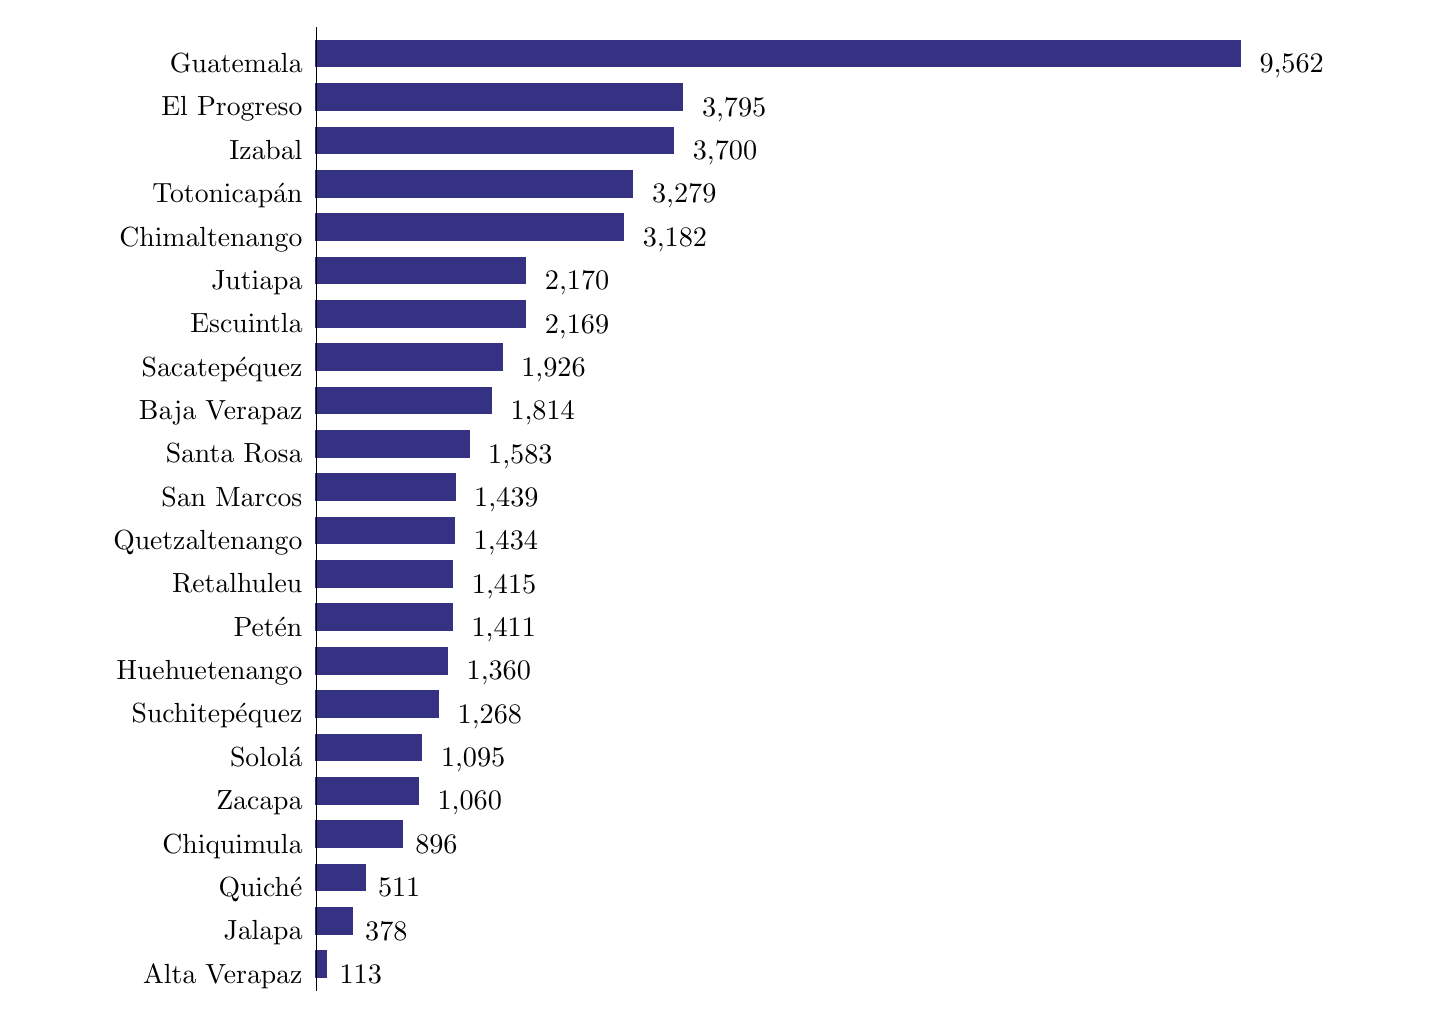
\begin{tikzpicture}[x=1pt,y=1pt, scale=1.75]% Created by tikzDevice version 0.12.4 on 2023-05-23 14:55:55
% !TEX encoding = UTF-8 Unicode
\definecolor{fillColor}{RGB}{255,255,255}
\path[use as bounding box,fill=fillColor,fill opacity=0.00] (0,0) rectangle (289.08,198.74);
\begin{scope}
\path[clip] (  0.00,  0.00) rectangle (289.08,198.74);

\path[] (  0.00,  0.00) rectangle (289.08,198.74);
\end{scope}
\begin{scope}
\path[clip] (  0.00,  0.00) rectangle (289.08,198.74);
\definecolor{drawColor}{RGB}{54,50,131}
\definecolor{fillColor}{RGB}{54,50,131}

\path[draw=drawColor,line width= 0.6pt,fill=fillColor] ( 59.47,  2.69) rectangle ( 61.73,  8.06);

\path[draw=drawColor,line width= 0.6pt,fill=fillColor] ( 59.47, 11.64) rectangle ( 67.02, 17.01);

\path[draw=drawColor,line width= 0.6pt,fill=fillColor] ( 59.47, 20.59) rectangle ( 69.67, 25.96);

\path[draw=drawColor,line width= 0.6pt,fill=fillColor] ( 59.47, 29.54) rectangle ( 77.36, 34.91);

\path[draw=drawColor,line width= 0.6pt,fill=fillColor] ( 59.47, 38.50) rectangle ( 80.63, 43.87);

\path[draw=drawColor,line width= 0.6pt,fill=fillColor] ( 59.47, 47.45) rectangle ( 81.33, 52.82);

\path[draw=drawColor,line width= 0.6pt,fill=fillColor] ( 59.47, 56.40) rectangle ( 84.78, 61.77);

\path[draw=drawColor,line width= 0.6pt,fill=fillColor] ( 59.47, 65.35) rectangle ( 86.62, 70.72);

\path[draw=drawColor,line width= 0.6pt,fill=fillColor] ( 59.47, 74.30) rectangle ( 87.64, 79.68);

\path[draw=drawColor,line width= 0.6pt,fill=fillColor] ( 59.47, 83.26) rectangle ( 87.72, 88.63);

\path[draw=drawColor,line width= 0.6pt,fill=fillColor] ( 59.47, 92.21) rectangle ( 88.10, 97.58);

\path[draw=drawColor,line width= 0.6pt,fill=fillColor] ( 59.47,101.16) rectangle ( 88.20,106.53);

\path[draw=drawColor,line width= 0.6pt,fill=fillColor] ( 59.47,110.11) rectangle ( 91.07,115.49);

\path[draw=drawColor,line width= 0.6pt,fill=fillColor] ( 59.47,119.07) rectangle ( 95.68,124.44);

\path[draw=drawColor,line width= 0.6pt,fill=fillColor] ( 59.47,128.02) rectangle ( 97.92,133.39);

\path[draw=drawColor,line width= 0.6pt,fill=fillColor] ( 59.47,136.97) rectangle (102.77,142.34);

\path[draw=drawColor,line width= 0.6pt,fill=fillColor] ( 59.47,145.92) rectangle (102.79,151.29);

\path[draw=drawColor,line width= 0.6pt,fill=fillColor] ( 59.47,154.88) rectangle (122.99,160.25);

\path[draw=drawColor,line width= 0.6pt,fill=fillColor] ( 59.47,163.83) rectangle (124.92,169.20);

\path[draw=drawColor,line width= 0.6pt,fill=fillColor] ( 59.47,172.78) rectangle (133.33,178.15);

\path[draw=drawColor,line width= 0.6pt,fill=fillColor] ( 59.47,181.73) rectangle (135.22,187.10);

\path[draw=drawColor,line width= 0.6pt,fill=fillColor] ( 59.47,190.69) rectangle (250.34,196.06);
\definecolor{drawColor}{RGB}{0,0,0}

\path[draw=drawColor,line width= 0.1pt,line join=round] ( 59.47,-198.74) -- ( 59.47,397.48);

\node[text=drawColor,anchor=base west,inner sep=0pt, outer sep=0pt, scale=  1.02] at ( 64.40,  1.40) {  113};

\node[text=drawColor,anchor=base west,inner sep=0pt, outer sep=0pt, scale=  1.02] at ( 69.69, 10.35) {  378};

\node[text=drawColor,anchor=base west,inner sep=0pt, outer sep=0pt, scale=  1.02] at ( 72.34, 19.31) {  511};

\node[text=drawColor,anchor=base west,inner sep=0pt, outer sep=0pt, scale=  1.02] at ( 80.03, 28.26) {  896};

\node[text=drawColor,anchor=base west,inner sep=0pt, outer sep=0pt, scale=  1.02] at ( 84.65, 37.21) {1,060};

\node[text=drawColor,anchor=base west,inner sep=0pt, outer sep=0pt, scale=  1.02] at ( 85.35, 46.16) {1,095};

\node[text=drawColor,anchor=base west,inner sep=0pt, outer sep=0pt, scale=  1.02] at ( 88.80, 55.11) {1,268};

\node[text=drawColor,anchor=base west,inner sep=0pt, outer sep=0pt, scale=  1.02] at ( 90.64, 64.07) {1,360};

\node[text=drawColor,anchor=base west,inner sep=0pt, outer sep=0pt, scale=  1.02] at ( 91.66, 73.02) {1,411};

\node[text=drawColor,anchor=base west,inner sep=0pt, outer sep=0pt, scale=  1.02] at ( 91.74, 81.97) {1,415};

\node[text=drawColor,anchor=base west,inner sep=0pt, outer sep=0pt, scale=  1.02] at ( 92.11, 90.92) {1,434};

\node[text=drawColor,anchor=base west,inner sep=0pt, outer sep=0pt, scale=  1.02] at ( 92.21, 99.88) {1,439};

\node[text=drawColor,anchor=base west,inner sep=0pt, outer sep=0pt, scale=  1.02] at ( 95.09,108.83) {1,583};

\node[text=drawColor,anchor=base west,inner sep=0pt, outer sep=0pt, scale=  1.02] at ( 99.70,117.78) {1,814};

\node[text=drawColor,anchor=base west,inner sep=0pt, outer sep=0pt, scale=  1.02] at (101.94,126.73) {1,926};

\node[text=drawColor,anchor=base west,inner sep=0pt, outer sep=0pt, scale=  1.02] at (106.79,135.69) {2,169};

\node[text=drawColor,anchor=base west,inner sep=0pt, outer sep=0pt, scale=  1.02] at (106.81,144.64) {2,170};

\node[text=drawColor,anchor=base west,inner sep=0pt, outer sep=0pt, scale=  1.02] at (127.01,153.59) {3,182};

\node[text=drawColor,anchor=base west,inner sep=0pt, outer sep=0pt, scale=  1.02] at (128.94,162.54) {3,279};

\node[text=drawColor,anchor=base west,inner sep=0pt, outer sep=0pt, scale=  1.02] at (137.35,171.50) {3,700};

\node[text=drawColor,anchor=base west,inner sep=0pt, outer sep=0pt, scale=  1.02] at (139.24,180.45) {3,795};

\node[text=drawColor,anchor=base west,inner sep=0pt, outer sep=0pt, scale=  1.02] at (254.36,189.40) {9,562};

\path[] ( 59.47,  0.00) rectangle (250.34,198.74);

\path[] ( 59.47,  5.37) --
	(250.34,  5.37);

\path[] ( 59.47, 14.32) --
	(250.34, 14.32);

\path[] ( 59.47, 23.28) --
	(250.34, 23.28);

\path[] ( 59.47, 32.23) --
	(250.34, 32.23);

\path[] ( 59.47, 41.18) --
	(250.34, 41.18);

\path[] ( 59.47, 50.13) --
	(250.34, 50.13);

\path[] ( 59.47, 59.09) --
	(250.34, 59.09);

\path[] ( 59.47, 68.04) --
	(250.34, 68.04);

\path[] ( 59.47, 76.99) --
	(250.34, 76.99);

\path[] ( 59.47, 85.94) --
	(250.34, 85.94);

\path[] ( 59.47, 94.90) --
	(250.34, 94.90);

\path[] ( 59.47,103.85) --
	(250.34,103.85);

\path[] ( 59.47,112.80) --
	(250.34,112.80);

\path[] ( 59.47,121.75) --
	(250.34,121.75);

\path[] ( 59.47,130.70) --
	(250.34,130.70);

\path[] ( 59.47,139.66) --
	(250.34,139.66);

\path[] ( 59.47,148.61) --
	(250.34,148.61);

\path[] ( 59.47,157.56) --
	(250.34,157.56);

\path[] ( 59.47,166.51) --
	(250.34,166.51);

\path[] ( 59.47,175.47) --
	(250.34,175.47);

\path[] ( 59.47,184.42) --
	(250.34,184.42);

\path[] ( 59.47,193.37) --
	(250.34,193.37);

\path[] ( 59.47,  0.00) rectangle (250.34,198.74);
\end{scope}
\begin{scope}
\path[clip] (  0.00,  0.00) rectangle (289.08,198.74);

\path[] ( 59.47,  0.00) --
	( 59.47,198.74);
\end{scope}
\begin{scope}
\path[clip] (  0.00,  0.00) rectangle (289.08,198.74);
\definecolor{drawColor}{RGB}{0,0,0}

\node[text=drawColor,anchor=base east,inner sep=0pt, outer sep=0pt, scale=  1.00] at ( 56.72,  1.46) {Alta Verapaz };

\node[text=drawColor,anchor=base east,inner sep=0pt, outer sep=0pt, scale=  1.00] at ( 56.72, 10.42) {Jalapa };

\node[text=drawColor,anchor=base east,inner sep=0pt, outer sep=0pt, scale=  1.00] at ( 56.72, 19.37) {Quiché };

\node[text=drawColor,anchor=base east,inner sep=0pt, outer sep=0pt, scale=  1.00] at ( 56.72, 28.32) {Chiquimula };

\node[text=drawColor,anchor=base east,inner sep=0pt, outer sep=0pt, scale=  1.00] at ( 56.72, 37.27) {Zacapa };

\node[text=drawColor,anchor=base east,inner sep=0pt, outer sep=0pt, scale=  1.00] at ( 56.72, 46.22) {Sololá };

\node[text=drawColor,anchor=base east,inner sep=0pt, outer sep=0pt, scale=  1.00] at ( 56.72, 55.18) {Suchitepéquez };

\node[text=drawColor,anchor=base east,inner sep=0pt, outer sep=0pt, scale=  1.00] at ( 56.72, 64.13) {Huehuetenango };

\node[text=drawColor,anchor=base east,inner sep=0pt, outer sep=0pt, scale=  1.00] at ( 56.72, 73.08) {Petén };

\node[text=drawColor,anchor=base east,inner sep=0pt, outer sep=0pt, scale=  1.00] at ( 56.72, 82.03) {Retalhuleu };

\node[text=drawColor,anchor=base east,inner sep=0pt, outer sep=0pt, scale=  1.00] at ( 56.72, 90.99) {Quetzaltenango };

\node[text=drawColor,anchor=base east,inner sep=0pt, outer sep=0pt, scale=  1.00] at ( 56.72, 99.94) {San Marcos };

\node[text=drawColor,anchor=base east,inner sep=0pt, outer sep=0pt, scale=  1.00] at ( 56.72,108.89) {Santa Rosa };

\node[text=drawColor,anchor=base east,inner sep=0pt, outer sep=0pt, scale=  1.00] at ( 56.72,117.84) {Baja Verapaz };

\node[text=drawColor,anchor=base east,inner sep=0pt, outer sep=0pt, scale=  1.00] at ( 56.72,126.80) {Sacatepéquez };

\node[text=drawColor,anchor=base east,inner sep=0pt, outer sep=0pt, scale=  1.00] at ( 56.72,135.75) {Escuintla };

\node[text=drawColor,anchor=base east,inner sep=0pt, outer sep=0pt, scale=  1.00] at ( 56.72,144.70) {Jutiapa };

\node[text=drawColor,anchor=base east,inner sep=0pt, outer sep=0pt, scale=  1.00] at ( 56.72,153.65) {Chimaltenango };

\node[text=drawColor,anchor=base east,inner sep=0pt, outer sep=0pt, scale=  1.00] at ( 56.72,162.61) {Totonicapán };

\node[text=drawColor,anchor=base east,inner sep=0pt, outer sep=0pt, scale=  1.00] at ( 56.72,171.56) {Izabal };

\node[text=drawColor,anchor=base east,inner sep=0pt, outer sep=0pt, scale=  1.00] at ( 56.72,180.51) {El Progreso };

\node[text=drawColor,anchor=base east,inner sep=0pt, outer sep=0pt, scale=  1.00] at ( 56.72,189.46) {Guatemala };
\end{scope}
\begin{scope}
\path[clip] (  0.00,  0.00) rectangle (289.08,198.74);

\path[] ( 56.72,  5.37) --
	( 59.47,  5.37);

\path[] ( 56.72, 14.32) --
	( 59.47, 14.32);

\path[] ( 56.72, 23.28) --
	( 59.47, 23.28);

\path[] ( 56.72, 32.23) --
	( 59.47, 32.23);

\path[] ( 56.72, 41.18) --
	( 59.47, 41.18);

\path[] ( 56.72, 50.13) --
	( 59.47, 50.13);

\path[] ( 56.72, 59.09) --
	( 59.47, 59.09);

\path[] ( 56.72, 68.04) --
	( 59.47, 68.04);

\path[] ( 56.72, 76.99) --
	( 59.47, 76.99);

\path[] ( 56.72, 85.94) --
	( 59.47, 85.94);

\path[] ( 56.72, 94.90) --
	( 59.47, 94.90);

\path[] ( 56.72,103.85) --
	( 59.47,103.85);

\path[] ( 56.72,112.80) --
	( 59.47,112.80);

\path[] ( 56.72,121.75) --
	( 59.47,121.75);

\path[] ( 56.72,130.70) --
	( 59.47,130.70);

\path[] ( 56.72,139.66) --
	( 59.47,139.66);

\path[] ( 56.72,148.61) --
	( 59.47,148.61);

\path[] ( 56.72,157.56) --
	( 59.47,157.56);

\path[] ( 56.72,166.51) --
	( 59.47,166.51);

\path[] ( 56.72,175.47) --
	( 59.47,175.47);

\path[] ( 56.72,184.42) --
	( 59.47,184.42);

\path[] ( 56.72,193.37) --
	( 59.47,193.37);
\end{scope}
\begin{scope}
\path[clip] (  0.00,  0.00) rectangle (289.08,198.74);

\path[] ( 59.47,  0.00) --
	(250.34,  0.00);
\end{scope}
\end{tikzpicture}}{INE - Censo 2018}